\documentclass[a4paper, 10pt]{article}        %\documentclass{} slides report proc book 
\usepackage[margin=1in]{geometry}
\usepackage{indentfirst}
\usepackage[]{graphicx}
\usepackage{standalone}
\usepackage[hyperref]{xcolor}
\definecolor{teal}{RGB}{0, 128, 128}


\usepackage{hyperref, xcolor}
\hypersetup{
        colorlinks = true,
        allcolors={teal},
        linkcolor={teal}
       %urlcolor=[rgb]{0,128,128},
     }
\title{Viral Beacon Data freeze 20200524 - Variant files statistics}     

\begin{document}
\date{}
\maketitle
%\author{{\color{teal}Claudia Vasallo}}


% General Statistics
\section{Summary stats}
%Statistics are calculated using \href{https://github.com/clauw87/virusbeacon/blob/raw_ideas/filters.pdf}{\texttt{Filters}}.

\begin{enumerate}

\item  38009 variant files %(from  X total samples and total ) % 1473 + 3925 (- 26 common to illumina) 
%\item   37942 samples % 5260  + 3053 + 29629 %(from  X total samples and total ) % 1473 + 3925 (- 26 common to illumina) 
%\item  X virus isolates %(from  X total samples and total ) % 1473 + 3925 (- 26 common to illumina) 


%%%%%% OVERALL PIES %%%%%%
% GEO LOC  >SRA, ENA AND GISAID


% RESOURCES: SRA, ENA AND GISAID
% VARIANT FILES TYPE: RAW/ CONSENSUS
\item[] \textsl{by data type} : \\
intra-host=1497 \\
consensus=36512\\


\item[] \textsl{by data resource}: \\
SRA: 4650 (raw sequence files) \\
ENA=3053 (consensus sequence files)\\
GISAID=29629 (consensus sequence files)

   \begin{figure}[!htb]
     \centering
     
\includegraphics[width=0.4\textwidth]{all_type_pie.pdf}
       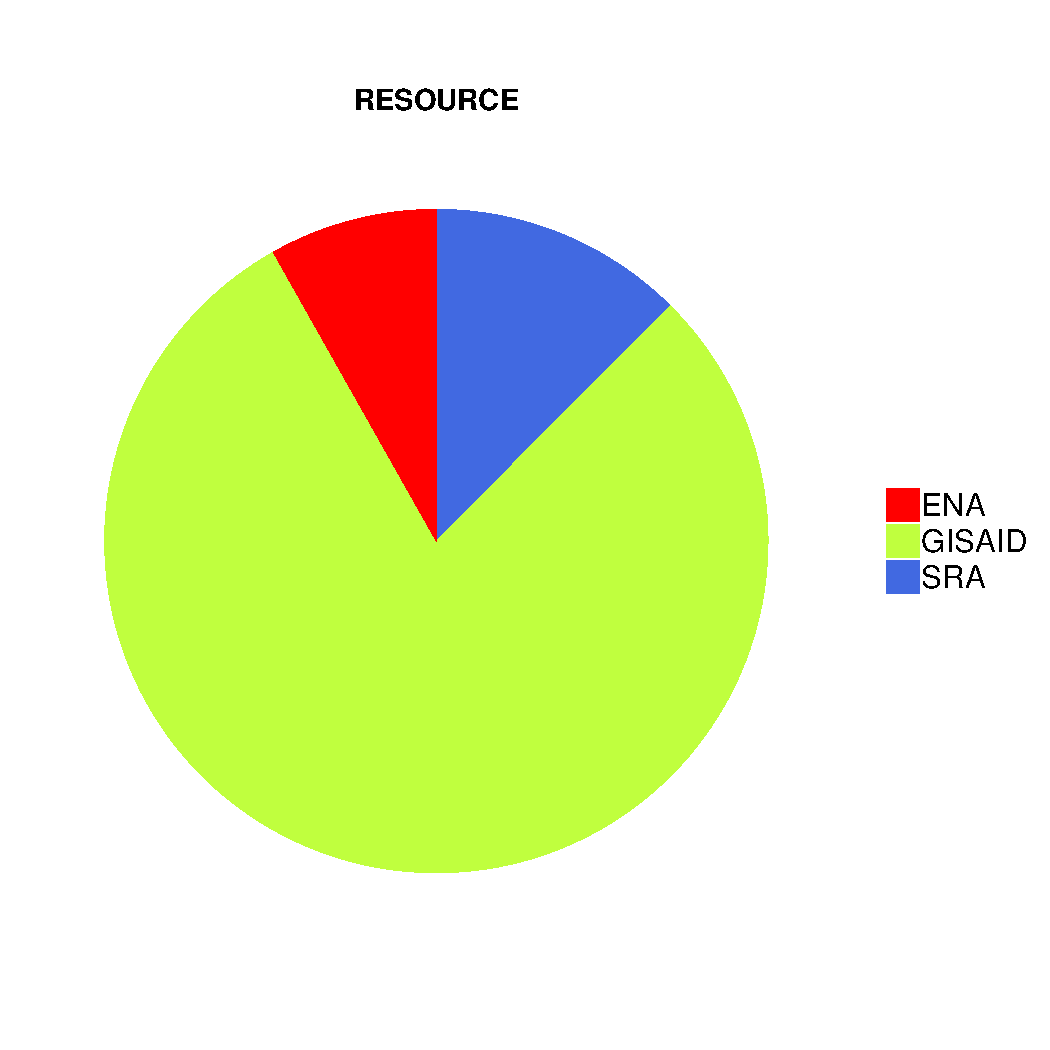
\includegraphics[width=0.4\textwidth]{all_reso_pie.pdf}
     %\caption{Distribution of variant files by type and resource}
     \label{fig:illu}
 \end{figure}


%GWH=?\\
% SEQ TECHNOLOGY - PIPELINE
\item[] \textsl{by resource \& pipeline}: \\
Illumina SRA-galaxy=1497 (raw/intrahost variants files) \\
ONT SRA-Medaka=3830 (consensus variants files)\\
%ION TORRENT SRA-Medaka=95 (consensus variants file-  warning: wrong maybe!),
ENA=3053 (consensus variants files)\\
GISAID=29629 (consensus variants files)\\

% SEQUENCING TECHNOLOGY, OVERALL AND SPLIT BY RESOURCE>SRA, ENA AND GISAID

\item[] \textsl{by sequencing technology}: \\
SRA: Illumina=1497, Oxford Nanopore=3830,  \\ %IonTorrent=95,
ENA, GISAID: (many, mixes, see by resource stats) \\
%\item[\textsl{option}] Split by sequencing platform model
%\item[\textsl{option}] Split by sequencing library layout          



% GEO LOC
% COL DATE
% AGE GROUPS
% SEX
% SAMPLE SOURCE



%%%%%% OVERALL STACKED BAR BLOTS %%%%%%
\item 37696(*) samples  (SRA: 5260, ENA: 3053, GISAID: 29629) % (37942) 
%* unique samples based on common samples that are cross-references
(*) This number is based on unique sample id and common samples that are cross-referenced across the databases.  
\item[] \textsl{Note}: Some variant files have the same samples  as source: 24 SRA samples have more than one Illumina run, 17 SRA samples have more than one ONT run, and 26 SRA samples have both Illumina and ONT runs. There are 246 samples are common to SRA (ONT) and GISAID datasets. We don't know if some sample counts are also common to SRA (Illumina) and GISAID, or common to ENA and GISAID,  or common to SRA and ENA.



 \end{enumerate}
 
 \newpage
\section{Stats variant files metadata by resources (SRA, ENA, GISAID)}


% GEO LOC  >SRA, ENA AND GISAID
   \begin{figure}[!htb]
     \centering
       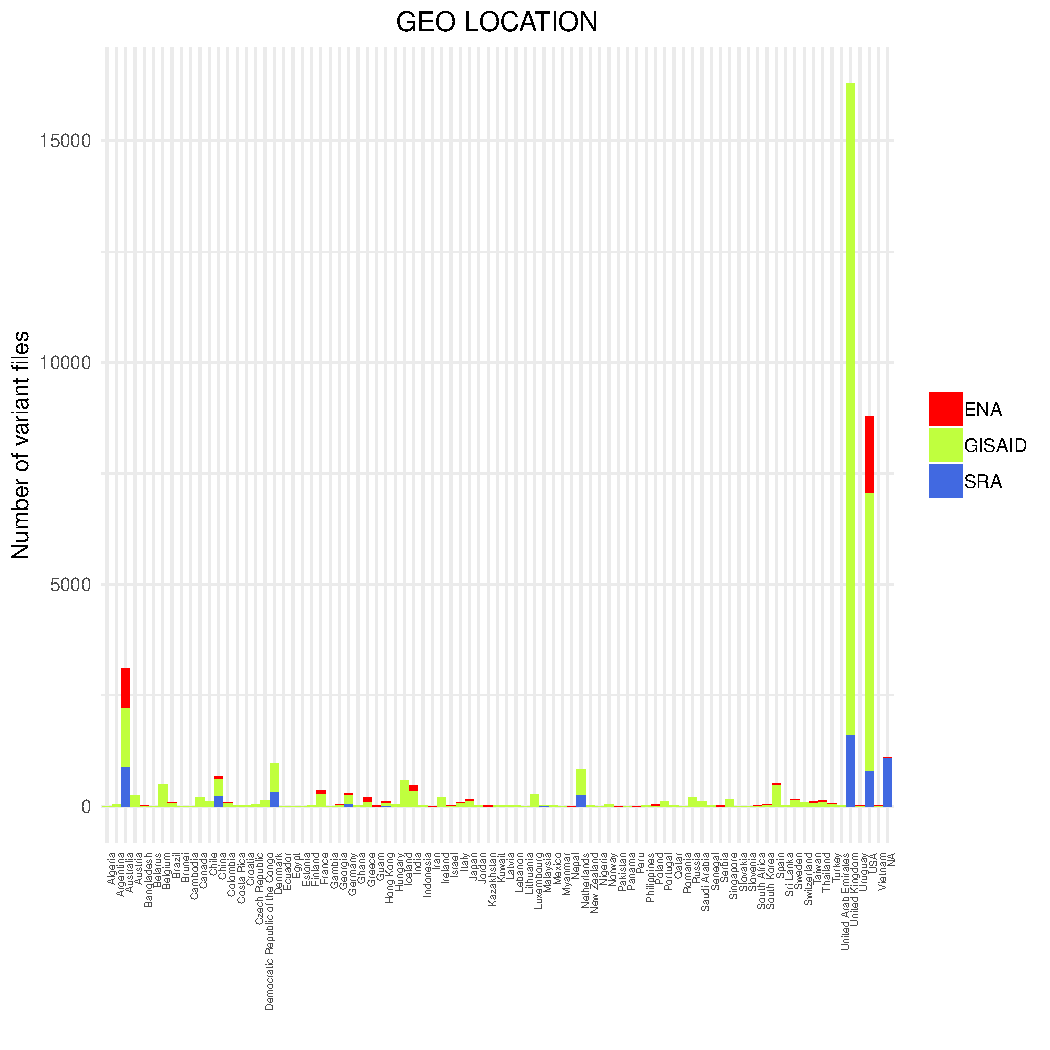
\includegraphics[width=1\textwidth]{all_loc_res.pdf}
     \caption{Distribution of variant files by country by resource}
     \label{fig:illu}
 \end{figure}



% COL DATE > SRA, ENA AND GISAID
   \begin{figure}[!htb]
     \centering
       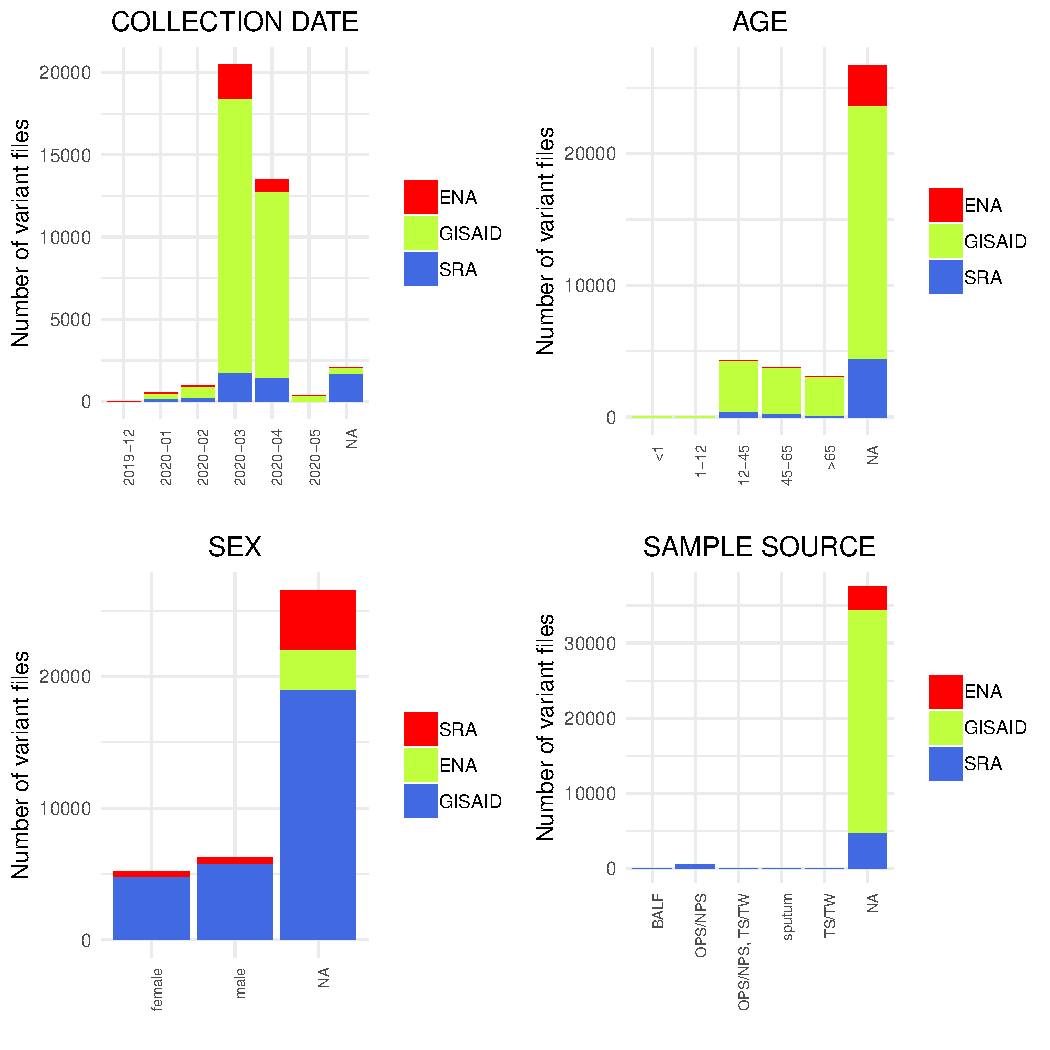
\includegraphics[width=1\textwidth]{all_grid.pdf}
     \caption{Distribution of variant files by collection date, host age, host sex, sample source by resource}
     \label{fig:illu}
 \end{figure}




 
 % SEQ TECH  >SRA, ENA AND GISAID
   \begin{figure}[!htb]
     \centering
       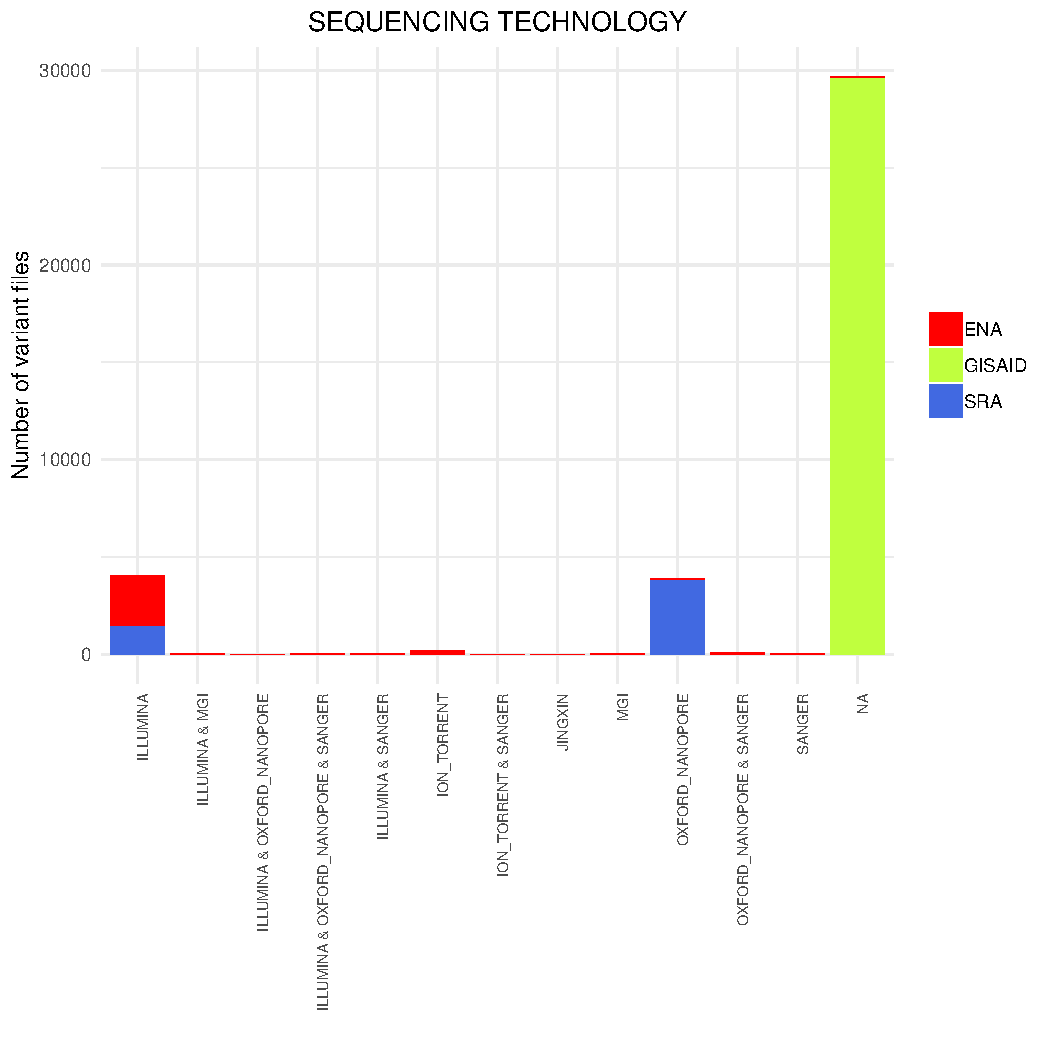
\includegraphics[width=1\textwidth]{all_plat_res.pdf}
     \caption{Distribution of variant files by sequencing technology by resource}
     \label{fig:illu}
 \end{figure}

 

 
 


\end{document}



% COL DATE > SRA, ENA AND GISAID
   \begin{figure}[!htb]
     \centering
       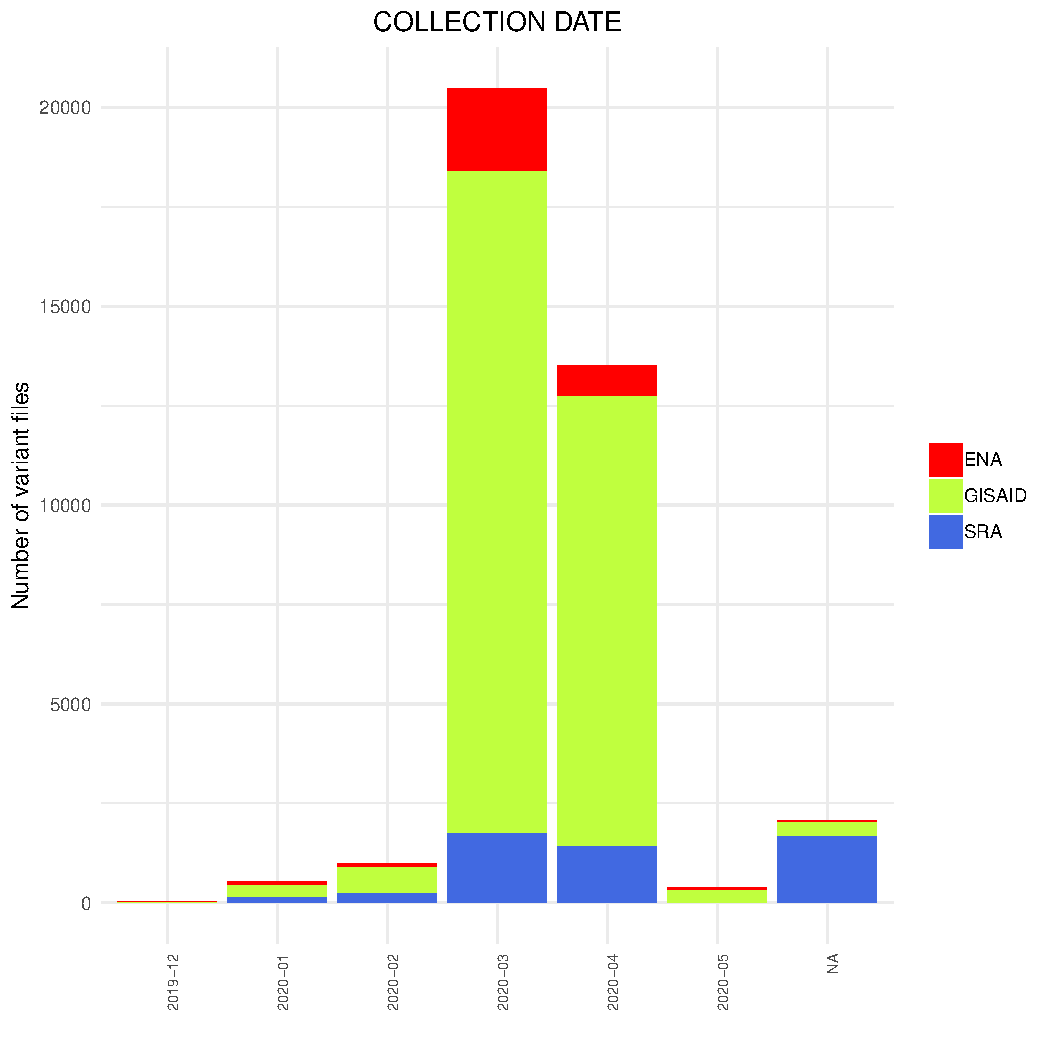
\includegraphics[width=1\textwidth]{all_date_res.pdf}
     \caption{Distribution of variant files by collection date by resource}
     \label{fig:illu}
 \end{figure}



% HOST AGE  >SRA, ENA AND GISAID
   \begin{figure}[!htb]
     \centering
       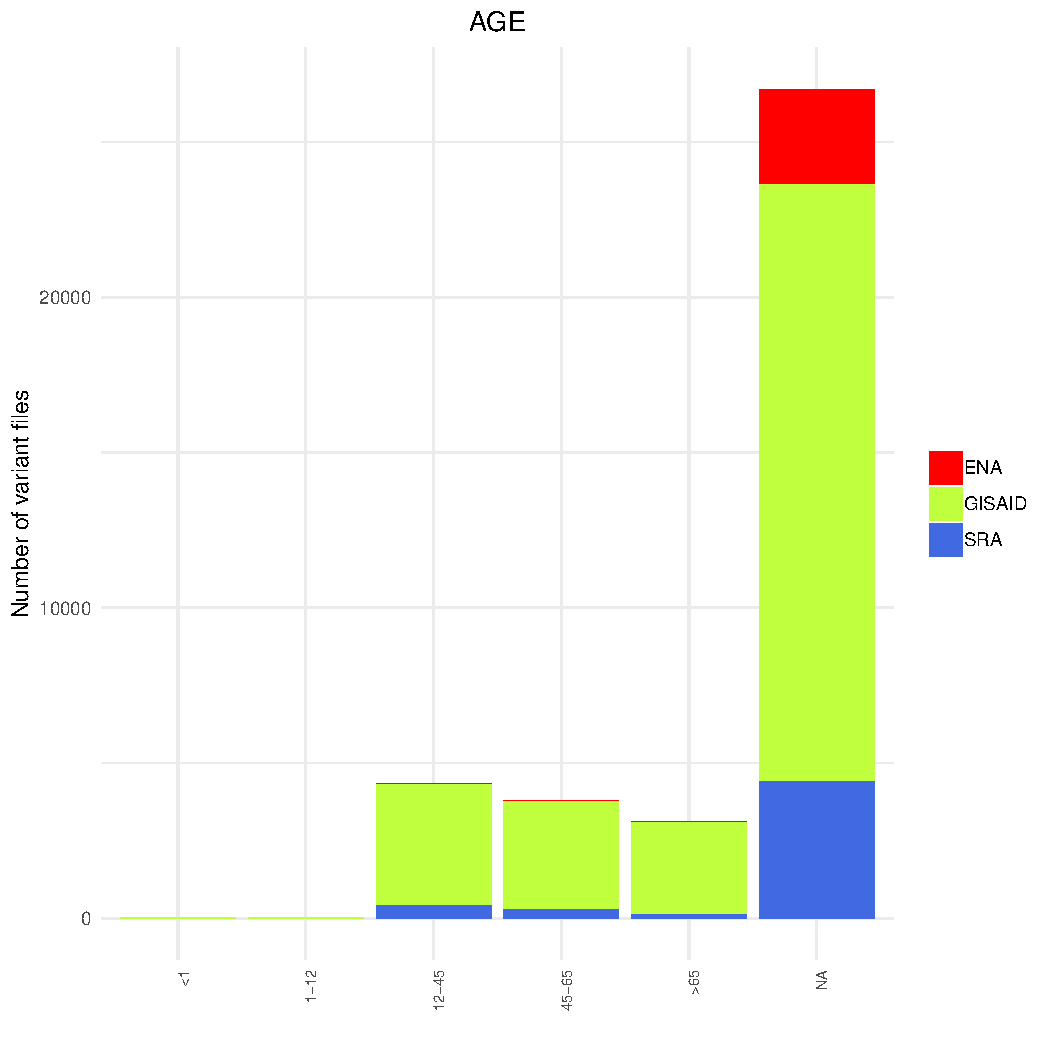
\includegraphics[width=1\textwidth]{all_age_res.pdf}
     \caption{Distribution of variant files by host age by resource}
     \label{fig:illu}
 \end{figure}




% HOST SEX  >SRA, ENA AND GISAID
   \begin{figure}[!htb]
     \centering
       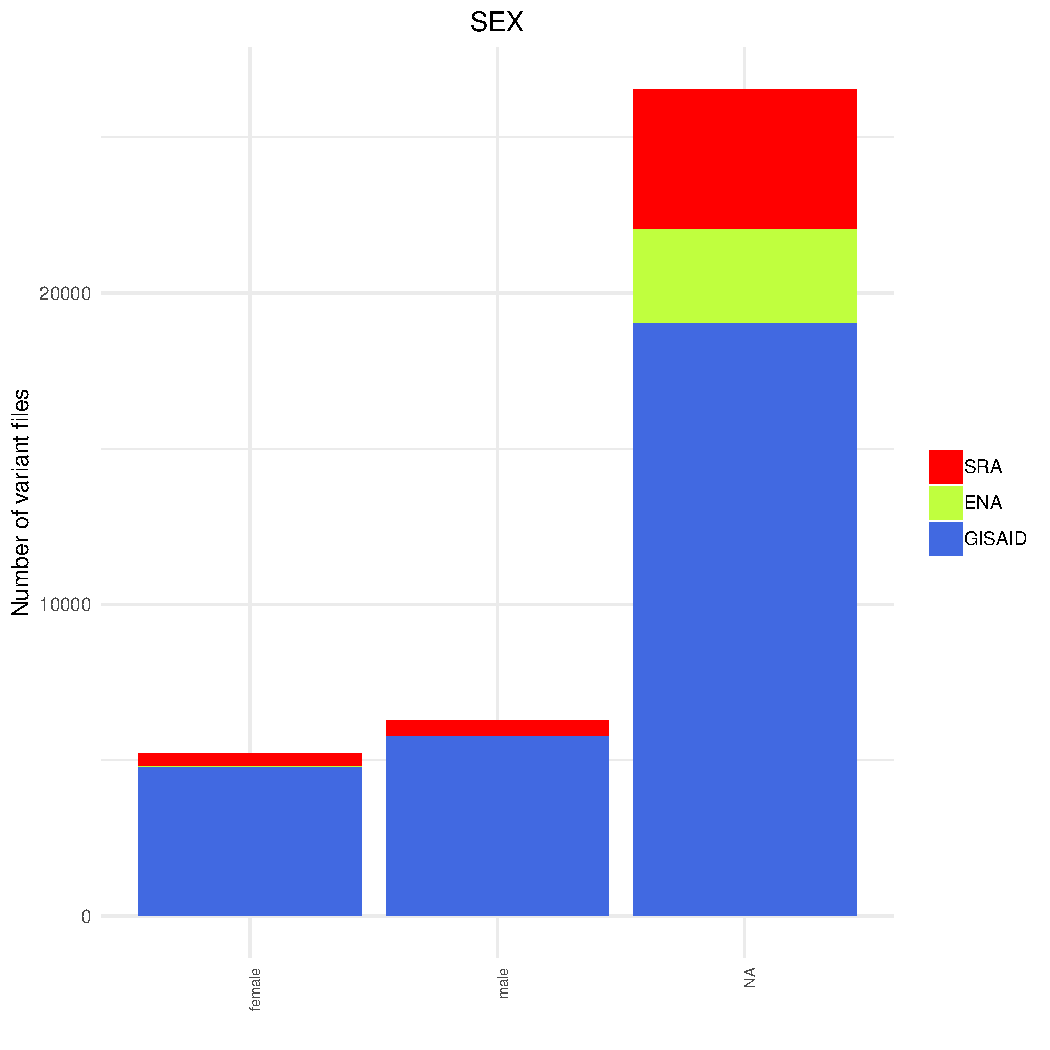
\includegraphics[width=1\textwidth]{all_sex_res.pdf}
     \caption{Distribution of variant files by host sex by resource}
     \label{fig:illu}
 \end{figure}
 

 
% SAMPLE SOURCE  >SRA, ENA AND GISAID
   \begin{figure}[!htb]
     \centering
       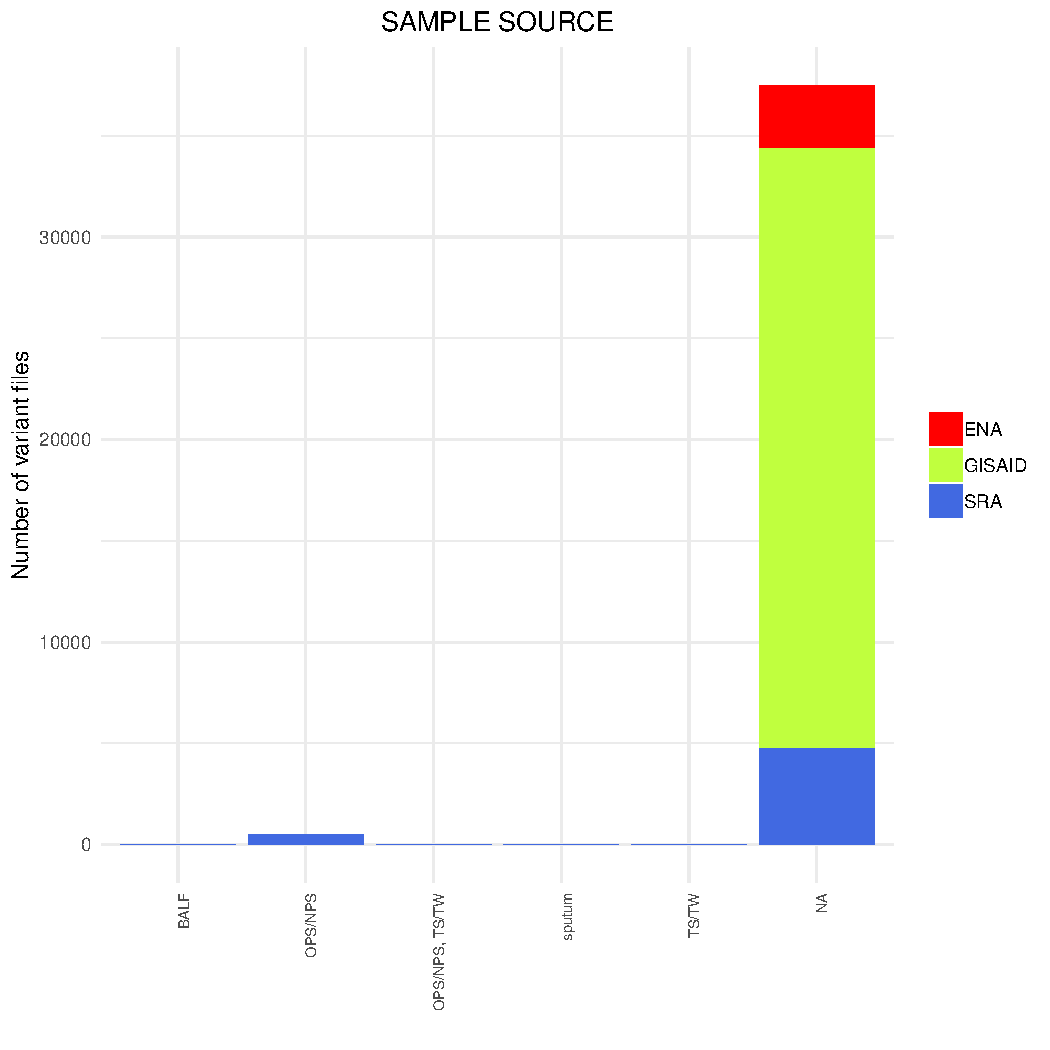
\includegraphics[width=1\textwidth]{all_sample_res.pdf}
     \caption{Distribution of variant files by sample source by resource}
     \label{fig:illu}
 \end{figure}

